% 47-15(47쪽) — 두 곡선 $y=\log_2 2x$, $y=\log_2 \dfrac{x}{2}$ 와 직선 $y=k$, 네 점 A·B·C·D, 색칠한 부분(원문 「오른쪽 그림」).
% 스캔 화질이 낮아 TikZ 로 다시 그림. 라벨은 원문에 있는 것만 — $y=k$ · A · B · C · D · 두 곡선 이름 · $\pt{O}$ · $x$ · $y$.
% 눈금 수치는 원문에도 없다. $\seg{AB}=4$ 와 넓이(답)는 그림에서 읽히지 않게 길이를 적지 않았다.
\begin{tikzpicture}[line width=0.6pt, x=0.45cm, y=0.42cm, >=stealth]
  \fill[green!18] plot[domain=1:4, samples=80, smooth] (\x, {ln(\x)/0.693147+1}) -- plot[domain=4:1, samples=80, smooth] (\x, {ln(\x)/0.693147-1}) -- cycle;
  \draw[->, line width=0.7pt] (-0.8,0) -- (6.0,0) node[below=1pt, font=\small] {$x$};
  \draw[->, line width=0.7pt] (0,-2.6) -- (0,4.1) node[left=1pt, font=\small] {$y$};
  \draw[line width=0.5pt] (-0.85,1) -- (5.2,1);
  \draw[domain=0.30:5.6, samples=140, smooth] plot (\x, {ln(\x)/0.693147+1});
  \draw[domain=0.42:5.6, samples=140, smooth] plot (\x, {ln(\x)/0.693147-1});
  \draw (1,1) -- (1,-1);
  \draw (4,1) -- (4,3);
  \draw[line width=0.35pt] (1,0.68) -- (1.3,0.68) -- (1.3,1);
  \draw[line width=0.35pt] (4,1.32) -- (3.7,1.32) -- (3.7,1);
  \node[anchor=east, font=\small] at (-0.95,1) {$y=k$};
  \node[anchor=south east, font=\small] at (0.95,1.08) {$\pt{A}$};
  \node[anchor=south west, font=\small] at (4.12,1.02) {$\pt{B}$};
  \node[anchor=west, font=\small] at (1.08,-1.22) {$\pt{C}$};
  \node[anchor=south west, font=\small] at (4.05,3.02) {$\pt{D}$};
  \node[anchor=south west, font=\small] at (0.75,3.55) {$y=\log_2 2x$};
  \draw[->, line width=0.3pt] (1.60,3.50) to[bend left=20] (1.86,2.02);
  \node[anchor=north, font=\small] at (3.50,-1.35) {$y=\log_2 \dfrac{x}{2}$};
  \draw[->, line width=0.3pt] (2.55,-1.28) to[bend right=20] (1.84,-0.22);
  \node[anchor=north east, font=\small] at (-0.04,-0.04) {$\pt{O}$};
\end{tikzpicture}
